\chapter{自旋交换相互作用体系少体精确解}\label{chap:kondo}

受到最近在超冷碱土金属平台中模拟近藤物理的实验以及理论进展的启发,采用严格对角化的数值方法,我们精确地研究了一维谐振子势场下一个局域磁性杂质与一个以及两个巡游费米子在自旋交换相互作用支配下的1+1以及1+2少体体系的能谱结构。在1+1少体体系中,我们发现对应于不同的铁磁、反铁磁耦合,少体精确解中的attractive branch与repulsive branch具有不同的磁性结构。对于1+2少体体系,在反铁磁耦合下的attractive branch中我们发现了类似于多体物理中的近藤屏蔽效应。进一步地,我们在反铁磁耦合体系中发现了一系列铁磁repulsive branch,它们与其他的attractive branch正交,并且其波函数拥有良好的自旋电荷分离的特点。最后,我们还简单探讨了实际体系中经常带有的接触相互作用带来的影响以及向多体体系的推广。我们的结果尝试从少体的角度发觉带有自旋交换相互作用影响的体系所独有的内禀物理特性,并期待可以在未来的超冷原子实验中得到实现与探索。

在~\ref{sec:spex-intro}~节中,我们介绍这一工作的背景和动机。在~\ref{sec:spex-model}~节中,我们介绍考虑的少体模型以及求解的数值方法。在~\ref{sec:spex-result}~节中,我们讨论得到结果并揭示其物理图像。在~\ref{sec:spex-summary}~节中,我们总结我们的结果并做后续研究的展望。

\section{引言}\label{sec:spex-intro}
在本论文的第一章里面~\ref{sec:spin-exchange}~中我们系统的介绍了自旋交换相互作用在超冷碱土金属原子中的研究进展。总体来讲,利用最外层2个电子的中性原子的基态${}^1S_0$与激发态${}^3P_0$来组成两轨道体系,整个原子的核自旋作为每个粒子的自旋自由度。不同轨道之间的自旋交换相互作用由实验所证实,其中裸的铁磁交换相互作用由${}^{173}$Yb\cite{scazza2014observation,cappellini2014direct,pagano2015strongly,hofer2015observation}与${}^{87}$Sr\cite{zhang2014spectroscopic}原子实现,而裸的反铁磁交换相互作用由${}^{171}$Yb\cite{ono2019antiferromagnetic}原子实现。通过使用束缚诱导共振技术,我们可以方便地低维度下体系的自旋交换相互作用的强度。这种调节已由理论和实验所证实\cite{zhang2016kondo,cheng2017enhancing,zhang2018control,ji2018confinement,zhang2020tight,zhang2020controlling,riegger2018localized}。进一步地,在近藤物理模拟中起关键作用的局域磁性杂质可以借由“魔法”频率光晶格来实现,其原理在于选取合适频率的激光形成光晶格,这种特殊的光晶格利用不同原子态的交流极化率来有选择性的使${}^3P_0$态的原子被束缚住,而${}^1S_0$态的原子则可以自由运动\cite{riegger2018localized,barber2008optical}。上述实验技术与理论计算的进展使得冷原子平台模拟多体近藤物理不再遥远。

不止于此,基于目前的研究进展,我们发现已经可以将目光聚集在少体体系。不同于多体体系,少体体系其独有的理论精确解为理解其中的物理提供坚实的基础。其中简洁的物理图像不仅为少体体系独有,而且为理解与表征多体体系提供丰富的线索。在本文的~\ref{sec:fewbody}~里面我们讨论了相关的背景,{\color{red} 待补充 }


综上,我们发现带有自旋交换相互作用的少体体系亟需系统的研究。因此在这一章节中,我们采用严格对角化的数值方法,系统地求解了1维简谐势场下带有自旋交换相互作用的1+N少体体系:
\begin{equation}\label{eq:sp-ex}
    \adddotsbeforeeqnnum%
    \hat{U}_{ex} = J\cdot\sum_{j=1}^{N}\hat{\Vector{S}}_j\cdot\hat{\Vector{S}}\cdot \delta(x_j)
\end{equation}
其中前面的1为局域带自旋1/2的磁性杂质(自旋算符为$\hat{\Vector{S}}$),位于原点处。后部面的N代表带自旋1/2的巡游费米子(自旋算符为$\hat{\Vector{S}}_j$),在本文中我们研究$N=1,2$。我们考虑杂质与费米子之间各向同性的铁磁与反铁磁海森堡耦合,其耦合强度可以调节。早在1980年代,描述一维连续空间里的费米子与局域自旋杂质体系的多体近藤模型就可用贝特假设的办法严格求解\cite{andrei1983solution},不过其前提在于假设费米子的色散关系为线性($\epsilon_k\propto k$),并带有可重整化的cut off。在这个假设下得到的结果,只有当费米海附近的费米子被自旋杂质散射时才成立,这对应若耦合极限附近。作为对比,在我们这一章节讨论当中,我们求解从弱到强整个相互作用区间的少体能谱与波函数,旨在得到系统的少体物理结果,为多体体系的研究提供启发。


最终,我们的结果总结如下:在自旋交换相互作用支配下的少体体系,展示了不同于纯接触相互作用少体体系的新奇特性。attractive 与 repulsive branch 的磁性结构由自旋交换的铁磁$J<0$与反铁磁$J>0$所决定。重要地,对于1+2的少体体系,我们发现对于反铁磁耦合,基态的attractive branch展现出一种屏蔽效应,而铁磁耦合的attractive branck则没有这种屏蔽。进一步,我们在反铁磁耦合这边发现了一系列的铁磁upper branch激发态,这些特殊的铁磁branch与其它的attractive branch没有发生level avoid crossing,其波函数具有很好的自旋电荷分离的特性。这些新奇的现象都来自于自旋交换相互作用,相应的branch也很容易在碱土金属原子实验中去探测,最后我们还考虑了实际体系经常伴有的纯接触相互作用的影响,以及简单的从少体物理特性到多体物理特性的推广。

\section{模型与计算}\label{sec:spex-model}
我们首先详尽的给出考虑的1+1与1+2少体体系的哈密顿量,并结合具体的物理意义给出变分波函数,最终推导出用于数值求解的矩阵方程。
\subsection{1+N体系哈密顿量}
我们的1+N少体体系处于一维简谐势场中,一个局域的自旋杂质被固定在原点$x=0$处,仅有自旋自由度,空间自由度被冻结。N个巡游费米子在一维连续空间运动,坐标表象下其位置为$x_j,j=1,...,N$。巡游费米子与局域自旋杂质之间存在自旋交换相互作用,整个体系的哈密顿量为(我们在本章中取$\hbar=1$):
\begin{equation}\label{eq:spex-hamiltonian}
\adddotsbeforeeqnnum%
    \begin{split}
       	\hat{H}  &= \hat{H}_0 + \hat{U}_{ex}\\
		\hat{H}_0 &= \sum_{j=1}^{N} \left( -\frac{1}{2M} \frac{\partial^2}{\partial x_{j}^2}   +\frac{M\omega^2}{2}x_{j}^2 \right); \\
		\hat{U}_{ex} &= 2J\cdot\sum_{j=1}^N\delta(x_j){\hat{\Vector{S}}}_j\cdot {\hat{\Vector{S}}}.
    \end{split}
\end{equation}
其中$M$为巡游费米子的质量,$\omega$为谐振子的特征频率,$\hat{\Vector{S}}=(\hat{S}_{x},\hat{S}_{y},\hat{S}_{z})$与$\hat{\Vector{S}}_j=(\hat{S}_{jx},\hat{S}_{jy},\hat{S}_{jz})$分别代表杂质与费米子自旋算符。展开为产生湮灭场算符为:
\begin{equation}\label{eq:spex-field}
\adddotsbeforeeqnnum%
    \begin{split}
		\hat{S}_{jx} &= \frac{1}{2}(\hat{\psi}_{\uparrow}^{\dag}(x_j)\hat{\psi}_{\downarrow}(x_j)+\hat{\psi}_{\downarrow}^{\dag}(x_j)\hat{\psi}_{\uparrow}(x_j));\\
		\hat{S}_{jy} &= \frac{-i}{2}(\hat{\psi}_{\uparrow}^{\dag}(x_j)\hat{\psi}_{\downarrow}(x_j)-\hat{\psi}_{\downarrow}^{\dag}(x_j)\hat{\psi}_{\uparrow}(x_j));\\
		\hat{S}_{jz} &= \frac{1}{2}(\hat{\psi}_{\uparrow}^{\dag}(x_j)\hat{\psi}_{\uparrow}(x_j)-\hat{\psi}_{\downarrow}^{\dag}(x_j)\hat{\psi}_{\downarrow}(x_j)).
    \end{split}
\end{equation}
其中$\hat{\psi}_{\sigma}^{\dag}(x)$为在x处产生一个自旋为$\sigma(\uparrow,\downarrow)$的费米子产生算符。在谐振子基矢下其展开式为:
\begin{equation}
\adddotsbeforeeqnnum%
	\hat{\psi}_{\sigma}^{\dag}(x)=\sum_m \hat{C}_{m\sigma}^{\dag} \phi_m(x).
\end{equation}
其中$\hat{C}_{m\sigma}^\dagger$是产生一个处于第$m$个简谐振子能级的带有自旋$\sigma$费米子的产生算符,该能级的本征波函数在坐标表象下记为$\hat{\phi}_m(x)$,本征能量为$E_m = (m+\frac{1}{2})\omega$。在这套完备的谐振子基矢下系统的哈密顿量(\ref{eq:spex-hamiltonian})可以重新写为二次量子化形式:
\begin{equation}
	\begin{split}
		\hat{H} &= \sum_{m\sigma}E_m \hat{C}_{m\sigma}^\dagger \hat{C}_{m\sigma} + \sum_{m,n} \hat{V}_{mn} ( \hat{C}_{m\uparrow}^\dagger  \hat{C}_{n\downarrow} \hat{S}_- + h.c. \\
     	& +   (\hat{C}_{m\uparrow}^\dagger  \hat{C}_{n\uparrow}-\hat{C}_{m\downarrow}^\dagger  \hat{C}_{n\downarrow}) \hat{S}_{z} ), \label{eq:H2}\\
\end{split}
\end{equation}
其中$V_{mn} = J\phi_m(0)\phi_n(0)$是自旋交换相互作用$\hat{V}_{ex}$导致的$m,n$本征态之间跃迁的矩阵元。我们记$|\Uparrow\rangle$ 与$|\Downarrow\rangle$为局域杂质的自旋态,因此我们有$S_+=|\Uparrow\rangle\langle \Downarrow|$,$S_-=|\Downarrow\rangle\langle \Uparrow|$,而$S_z=(|\Uparrow\rangle\langle \Uparrow|-|\Downarrow\rangle\langle \Downarrow|)/2$。我们可以清楚得看到自旋交换过程是由(\ref{eq:H2})中括号里面的前两项实现的。

接下来我们给出用于具体求解少体能谱的计算公式。包括1+1与1+2自旋交换作用少体体系。

\subsection{一个杂质与一个费米子}
由于哈密顿量(\ref{eq:H2})依然具有自旋$SU(2)$旋转对称性。1+1少体体系按照一个杂质与一个费米子系统总的自旋$\hat{\Vector{S}}_{tot}$划分为自旋三重态通道($\hat{\Vector{S}}_{tot}=1$)与自旋单重态通道($\hat{\Vector{S}}_{tot}=0$)。每个独立的通道都是自旋算符的本征态。因此我们有每个通道的有效描述:
\begin{equation}
U_{s,t}(x_1)=\gamma_{s,t}\delta(x_1).
\end{equation}
其中单重态($singlet$)通道下费米子与杂质的有效耦合强度为$\gamma_s = \frac{-3J}{2}$,三重态($triplet$)通道下费米子与杂质的有效耦合强度为$\gamma_t = \frac{J}{2}$。

为了在同一个变分波函数中包含单重态通道与三重态通道的共同表达式,我们将波函数取在($S_{tot,z}=0$)的封闭子希尔伯特空间中:
\begin{equation}
	|\Psi\rangle_2=\sum_m \left( \phi_m^1 \hat{C}_{m\uparrow}^\dagger|0\rangle \Downarrow+ \phi_m^2 \hat{C}_{m\downarrow}^\dagger|0\rangle \Uparrow \right).
\end{equation}
其中$|0\rangle$是具有0个费米子的真空态。将波函数带入到薛定谔方程:
\begin{equation}
	\hat{H} |\Psi \rangle_2 = E |\Psi\rangle_2,
\end{equation}
我们得到如下的耦合方程组
\begin{equation}
    \begin{split}
      (E-E_m) \phi^1_m &= \sum_p (V_{mp}\phi^2_p-\frac{1}{2}V_{mp}\phi^1_p )\\
      (E-E_m) \phi^2_m &= \sum_p (V_{mp}\phi_p^1 -\frac{1}{2}V_{mp}\phi^2_p).
    \end{split}
\end{equation}
我们从中可以看到这组耦合方程有两类解,其中一类是:
\begin{equation}
    \phi^1_m=\phi^2_m \propto \frac{\phi_m(0)}{E-E_m},
\end{equation}
容易发现,这类解对应的是一个自旋三重态,其能量$E(=E_t)$满足自洽方程:
\begin{equation}
      \frac{1}{\gamma_t} =  \sum_m \frac{|\phi_m(0)|^2}{E_t-E_m}. \label{eq_t}
\end{equation}
而另一类解对应的是一个自旋单重态:
    \begin{equation}
      \phi^1_m = -\phi^2_m\propto \frac{\phi_m(0)}{E_s-E_m},
    \end{equation}
其能量$E(=E_s)$满足自洽方程:
	\begin{equation}
      \frac{1}{\gamma_s} =  \sum_m \frac{|\phi_m(0)|^2}{E_s-E_m}. \label{eq_s}
    \end{equation}
进一步地,两个自洽方程(\ref{eq_t},\ref{eq_s})可以统一为一个方程:
    \begin{equation}
        -\frac{2\sqrt{\pi}}{\kappa_{s,t}} = B(-\frac{\rho_{s,t}}{2},\frac{1}{2}) 
    \end{equation}
其中$\kappa_{s,t} \equiv \gamma_{s,t}\sqrt{M/\omega}$, $\rho_{s,t} \equiv E_{s,t}/\omega-1/2$,而$B(x,y)$是特殊函数中的贝塔函数。

\subsection{一个杂质与两个费米子}
有了1+1体系的求解,我们进一步考虑如果再增加一个自由费米子变成1+2体系,会出现如何有趣的物理呢?对于1个杂质和2个费米子的三体体系,系统总的自旋$\hat{\Vector{S}}_{tot}$可以为$\hat{\Vector{S}}_{tot}=1/2$或者$\hat{\Vector{S}}_{tot}=3/2$。同样地出于统一求解两种总自旋态的角度,我们仍然考虑$S_{tot,z}=1/2$的封闭子希尔伯特空间。其变分波函数可以写为:
\begin{equation}\label{eq:wv3}
    |\Psi\rangle_3 = \sum_{mn} \left( \phi^1_{mn} \hat{C}_{m\uparrow}^\dagger \hat{C}_{n\uparrow}^\dagger \left|0\right> |\Downarrow\rangle + \phi^2_{mn}  \hat{C}_{m\uparrow}^\dagger \hat{C}_{n\downarrow}^\dagger \left|0\right> |\Uparrow\rangle \right).
\end{equation}
其中,出于对2个费米子交换反对称的考虑,我们要求$\phi^1_{mn} = -\phi^1_{nm}$。将变分波函数带入薛定谔方程:
\begin{equation}
  \hat{H} |\Psi \rangle_3 = E |\Psi\rangle_3,
\end{equation}
我们得到变分参数满足的耦合方程组:
\begin{equation}
    \begin{split}
        &\phi^1_{mn} = \frac{1}{E-E_m-E_n} \cdot \frac{1}{2} \cdot  \sum_{p}-V_{mp}\phi^2_{np}+V_{np}\phi^2_{mp} +V_{np}\phi^1_{pm}- V_{mp}\phi^1_{pn} \\
        &\phi^2_{mn} = \frac{1}{E-E_m-E_n} \sum_p V_{np}\phi^1_{mp}-V_{np}\phi^1_{pm}+ \frac{1}{2} V_{mp}\phi^2_{pn}- \frac{1}{2}V_{np}\phi^2_{mp}.
    \end{split}\label{eq:eq_3b}
\end{equation} 
可以看到$\phi^1_{mn}$的交换反对称性依然成立。
仔细观察耦合方程(\ref{eq:eq_3b})的结构,我们发现可以进一步引入辅助变量$F^1_m,F^2_m,F^3_m$来减小体系求解的自由度数目,其背后的物理来源于在自旋交换相互作用是$s$波接触势,其中的一费米子和杂质形成二聚体(dimer)态:
    \begin{equation}
        \begin{split}
        &F^1_n \equiv \sum_p\phi_p(0)\phi^1_{np} \\
        &F^2_n \equiv \sum_p\phi_p(0)\phi^2_{np} \\
        &F^3_n \equiv -\sum_p\phi_p(0)\phi^2_{pn}\\
        \end{split} \label{F}
    \end{equation}
然后我们把方程(\ref{eq:eq_3b})左右两边同时乘以$\phi_m(0)$并对$m$求和可以得到一组新的$F^(i)_m$所满足的耦合方程。为了使得其物理意义更加明显,我们对引入的辅助变量$F^(i)_m$做线性叠加组合为$\tilde{F}^{(1)}_m$:
\begin{equation}
    \begin{split}
        &\tilde{F}^{(1)}_n =-\frac{3}{2}F_n^{(1)} +\frac{3}{4}F_n^{(2)}\\
        &\tilde{F}^{(2)}_n =\frac{1}{2}F_n^{(1)}+\frac{1}{4}F_n^{(2)} \\
        &\tilde{F}^{(3)}_n =\frac{1}{2}F_n^{(3)}.
    \end{split} \label{tF}
\end{equation}
经过这样的线性变换之后,变分波函数(\ref{eq:wv3})有了很直观的原子-二聚体分离的波函数:
 \begin{equation}
    \begin{split}
        |\Psi\rangle_3 &=\sum_m \tilde{F}^{(1)}_m \left| m \uparrow \right> \left|d^{00}_{m}\right> + \tilde{F}^{(2)}_m \left|m\uparrow \right>  \left| d^{10}_{m}\right> +   \tilde{F}^{(3)}_m \left|m\downarrow\right> \left|d^{11}_{m}\right>\\
    \end{split}
    \end{equation}
其中不同内部磁性结构的二聚体波函数为:
\begin{eqnarray}
    \left|d^{11}_{m}\right> &=& \sum_p \frac{\phi_p(0)}{E-E_m-E_p} \left| p\uparrow \right>|\Uparrow\rangle ;\\
    \left|d^{10}_{m}\right> &=& \sum_p \frac{\phi_p(0)}{E-E_m-E_p} \frac{\left| p\uparrow \right>|\Downarrow\rangle+\left| p\downarrow \right>|\Uparrow\rangle}{\sqrt{2}} ;r\\
\left|d^{00}_{m}\right> &=& \sum_p \frac{\phi_p(0)}{E-E_m-E_p} \frac{\left| p\uparrow \right>|\Downarrow\rangle-\left| p\downarrow \right>|\Uparrow\rangle}{\sqrt{2}}. 
\end{eqnarray}
进一步地出于更加直观的考虑,我们将$\tilde{F}^{(1)}_m$满足的耦合方程写成矩阵的形式,为此我们引入$\tilde{F}^{(i)}\equiv (\tilde{F}^{(i)}_0,\tilde{F}^{(i)}_1,...)^T$,耦合方程(\ref{eq:eq_3b})最终被表达为:
     \begin{equation}
      \left(
        \begin{array}{ccc}
        \frac{1}{4} (e-2 q) 3 & \frac{3}{4} e  & \frac{-3}{4}  e  \\
        -\frac{1}{4}e & -\frac{1}{4} (e-2 q) & -\frac{1}{4} e  \\
        \frac{1}{2} e  & -\frac{1}{2} e  & \frac{1}{2} q  \\
        \end{array}
      \right)
        \left(
            \begin{array}{c}
                \tilde{F}^{(1)} \\
                \tilde{F}^{(2)} \\
                \tilde{F}^{(3)} \\
            \end{array}
        \right)
        =\frac{1}{J}
        \left(
            \begin{array}{c}
                \tilde{F}^{(1)} \\
                \tilde{F}^{(2)} \\
                \tilde{F}^{(3)} \\
            \end{array}
        \right)   \label{final_eq}
    \end{equation}  
其中$e,q$是大矩阵的子块,其矩阵元为:
\begin{equation}
    \begin{split}
      e_{mn} &= \frac{\phi_m(0) \phi_n(0)}{E-E_m-E_n}\\
      q_{mn} &= \delta_{mn}  \sum_p \frac{|\phi_p(0)|^2}{E-E_m-E_p}.   
    \end{split}
\end{equation}
可以看到$q$矩阵只出现在块对角的部分,这代表了费米子与局域杂质之间的相互作用形成一个二聚体的能量。而$e$则矩阵代表了二聚体与剩下的一个费米子之间的有效相互作用,这种少体关联是在1+1体系中所没有的。

在实际的数值计算中,我们选取足够大的谐振子能级上限来保证结果的收敛,在本文的计算中我们选取$N_c=100$,这时我们将要对角化的矩阵维度为$2N_c\times 3N_c$。此外我们还可以采用y一个小技巧,那就是对于我们选取不同的能量$E$固定,当$E$选定时,矩阵方程(\ref{final_eq})的左边矩阵是完全已知的,我们只需要一次严格对角化求出多有的本征值与本征矢量,其中对于每一个本征值的倒数就是对应的相互作用强度$J$,而本征波函数就是费米子-二聚体基矢下的波函数($\tilde{F}^{(1)}_0,...\tilde{F}^{(1)}_{N_c-1},\tilde{F}^{(2)}_0,...\tilde{F}^{(1)}_{N_c-1},\tilde{F}^{(3)}_0,...\tilde{F}^{(3)}_{N_c-1})^T$。

\section{结果}\label{sec:spex-result}
在本节中我们基于前面讨论1+1与1+2体系的哈密顿量与变分波函数,准确地求解了体系的能谱并加以分析。由于自旋交换相互作用哈密顿量依然保持有空间反演不变性,因此我们只考虑具有偶宇称的本征解,奇宇称的解不受自旋交换相互作用的影响。

\subsection{一个杂质与一个费米子}
在1+1体系里,通过选取自旋单重态与自旋三重态通道,
\begin{equation}
\begin{split}
    |s\rangle &= \frac{1}{\sqrt{2}}(|\uparrow\Downarrow - \downarrow\Uparrow\rangle),\\
    |t\rangle &= \frac{1}{\sqrt{2}}(|\uparrow\Downarrow + \downarrow\Uparrow\rangle),\\
\end{split}
\end{equation}

\begin{figure}[!htbp]
    \centering
    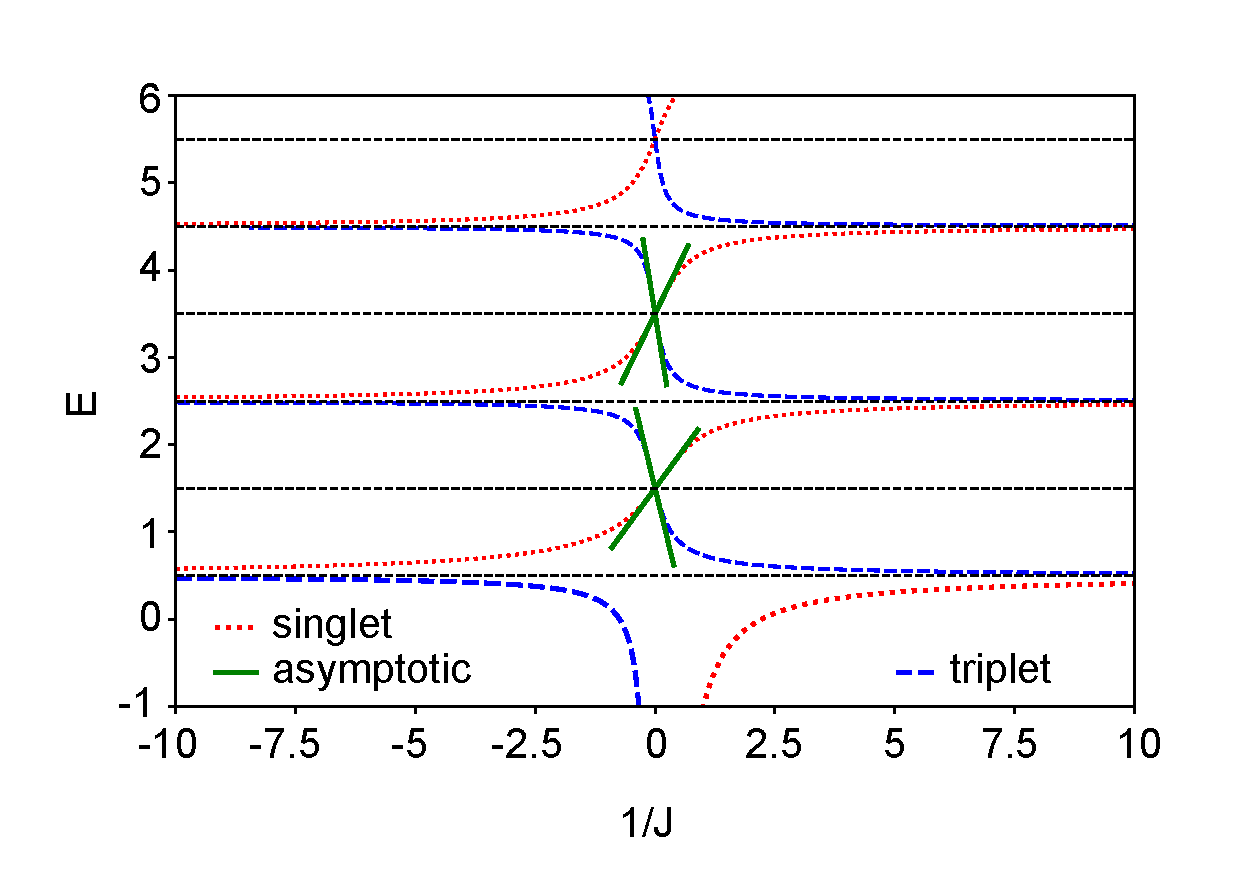
\includegraphics[width=0.7\textwidth]{fig1.pdf}
    \bicaption{一个杂质与一个费米子的1+1体系在$S_{tot,z}=0$子希尔伯特空间的能谱随自旋交换相互作用强度的变化。蓝色虚线(红色散点线)代表自旋三重态(自旋单重态)通道中的本征解。绿色实线代表强相互作用附近的微扰论渐近行为。其横纵坐标$E$与$J$的量纲为$\omega$与$\sqrt{\omega/M}$。}{(Color online). Energy spectrum of one fermion and one impurity in $S_{tot,z}=0$ subspace. The blue dashed (red dotted) lines show $E_t$ ($E_s$) for spin-triplet (singlet) eigen-states. The green solid line shows the asymptotic fitting to (\ref{asymptotic}) in strong coupling limit. Here the units of $E$ and $J$ are respectively $\omega$ and $\sqrt{\omega/M}$.}
    \label{fig:fig1}
\end{figure}

自旋交换部分已经被对角化,在各个通道内,自旋交换交换相互作用等价于纯的接触势,只不过接触势的符号受到自旋通道的影响。在如图~\ref{fig:fig1}~所示,我们展示了1+1两体中自旋单重态与自旋三重态通道的解,对应自洽方程(\ref{eq_t}与\ref{eq_s}),接下来我们来理解从这一能谱中得到的信息。



首先对于自旋单重态通道的解,对角化后的自旋交换相互作用对应强度为$\gamma_s=-3J/2$的接触相互作用,因此只有在$J>0$的时候,在散射态临界下面会有束缚态的产生。正如图~\ref{fig:fig1}~最下面的红色散点线所示,我们从$J=0$逐渐增大到$J=+\infty$,自旋单重束缚态的能量越来越低,在$J\to + \infty$附近,$E_s$渐近行为为$E_s\rightarrow -9J^2/8$。我们称这样的态为lower attractive branch。除了这支束缚态以外,我们发现其余的本征态在$J\to \pm \infty$的时候都趋近于有限大小的谐振子奇数能级,远远位于束缚态之上,我们称这样的一系列态为repulsive upper branch。如果我们逐渐放松谐振子的束缚程度,取$\omega\to 0$,我们会发现lower branch将变为一维接触势的唯一束缚态,而upper branch将变为一系列散射态。

对于自旋三重态通道的解,对角化后的自旋交换相互作用强度为$\gamma_t=J/2$,因此只有在$J<0$的时候才存在束缚态,如图~\ref{fig:fig1}~中最下面的蓝色虚线所示,当我们从$J=0$往负方向调节$J\to-\infty$时候,束缚态的能量不断降低,在$J\sim -\infty$附近其渐近行为是$E_t\rightarrow -J^2/8$。我们称这种态为lower attractive branch。类似地,在束缚态的上面,有一系列repulsive upper branch,它们的能量随$J\to-\infty$而趋近于谐振子的奇数能级处。

在$1/J=0$附近,我们看到不论单重态还是三重态的repulsive upper branch 能量都具有很好的线性行为,这表明此处可用微扰论来描述。具体地,我们以两体接触势$\gamma\delta(x)$为例(因为在三重态和多重态通道或中自旋交换相互作用被自动对角化为接触势),假设渐近行为是:
\begin{equation}
    E_m(\gamma) \simeq  (2m+1)\omega - \frac{A_m}{\gamma}.
\end{equation}
其中线性修正的系数$A_m$为待定。我们知道对于两体接触势来讲,势能部分哈密顿量带来波函数的边界条件,对任意$\gamma$:
\begin{equation}
    \gamma\psi_\gamma(0) = \frac{\psi'_\gamma(0)}{M}.
\end{equation}
根据Hellmann-Feynman定理,单参数哈密顿量能量对其参数的导数为:
\begin{equation}
\begin{split}
    \frac{dE(\gamma)}{d(1/J)} = -{}_\gamma\langle\psi| \gamma^2\delta(x) |\psi\rangle_\gamma
\end{split}
\end{equation}
其中$|\psi\rangle_\gamma$为接触势强度为$\gamma$时对应的某个本征解波函数,$E(\gamma)$为对应的本征能量,因此upper branch渐近行为的线性系数可由此计算:
\begin{equation}
\begin{split}
    A_m &= \lim_{\gamma\to \infty} -\frac{\partial E(\gamma)}{\partial \frac{1}{\gamma} }\\
    \quad &= \lim_{\gamma\to \infty} \int dx \gamma\psi_\gamma(x)\delta(x)\gamma\psi_\gamma(x) \\
    \quad &= \lim_{\gamma\to \infty} \gamma\psi_\gamma(0)\cdot \gamma\psi_\gamma(0). 
\end{split}
\end{equation}
最终我们得到单重态与三重态通道内upper branch的渐近行为:
\begin{equation}
E_{s/t,n} \simeq (2n+1)\omega -\frac{\phi^{'}_{2n+1}(0)^2}{M^2\gamma_{s/t}}. \label{asymptotic}
\end{equation}
其中$\phi'_n=d\phi_n(x)/dx$是谐振子本征波函数导数。在图~\ref{fig:fig1}~中,绿线代表了我们用此微扰论计算得到的线性行为,跟严格解的数值结果相一致。对应地,当$1/J=0$时候,系统的零阶未微扰波函数为\cite{zurn2012fermionization}:
\begin{equation}
|\Psi\rangle_{s/t,n} = \phi_{2n+1}(x) \cdot sgn(x)\left| s/t \right>, \label{asymptotic_wf}
\end{equation}
其中$|s\rangle = \frac{1}{\sqrt{2}}(|\uparrow\Downarrow - \downarrow\Uparrow\rangle)$,$|t\rangle = \frac{1}{\sqrt{2}}(|\uparrow\Downarrow + \downarrow\Uparrow\rangle)$ 具有自旋电荷分离的形式。
综上我们发现对于1+1体系,系统可以通过考虑各个通道中单粒子在接触势中的来图像方便地理解。最终的能谱也跟纯接触势中的1+1体系\cite{busch1998two}具有类似的行为。但是,随着我们在系统中再添加一个费米子,上面简单的单粒子图像便不再成立,能谱变得更加丰富,其中由自旋交换相互作用导致的新物理出现,这是完全不同于纯接触相互作用体系的新特性。在接下来的章节中们将对此详细介绍。

\subsection{一个杂质与两个费米子}

\begin{figure}[!htbp]
    \centering
    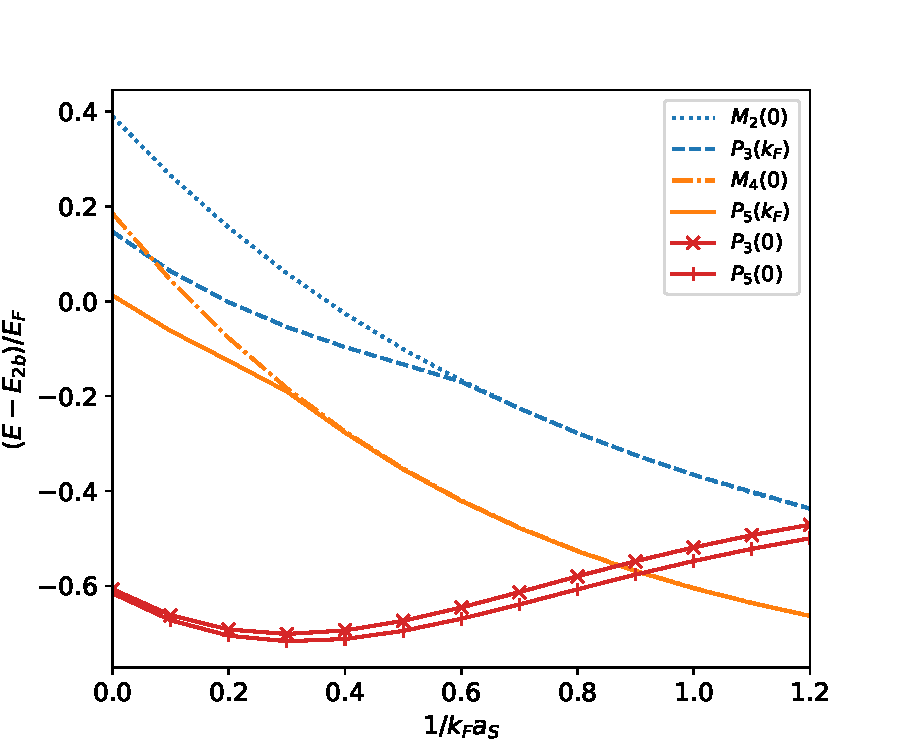
\includegraphics[width=0.7\textwidth]{fig2.pdf}
    \bicaption{一个杂质与两个个费米子的1+2体系在$S_{tot,z}=1/2$子希尔伯特空间的能谱随自旋交换相互作用与无自旋交换的接触相互作用强度的变化。a(1)代表的是带自旋交换相互作用1+2体系。我们用红色的点来标记其中特殊的$S_{tot=3/2}$的铁磁态。剩下的态都是$S_{tot}=1/2$的态。a(2)代表的是带纯接触势的1+2体系的能谱。其中$E$与$J$的量纲为$\omega$与$\sqrt{\omega/M}$。}{(Color online).(a1) Energy spectrum of two fermions and one impurity with spin-exchange interaction in the $S_{tot,z}=1/2$ subspace. The FM states with $S_{tot}=3/2$ are highlighted by red color, and the rest are all with total spin $S_{tot}=1/2$. (a2) Same as (a1) except that the interaction between fermions and impurity is a pure contact type without spin-exchange, see text. }
    \label{fig:fig2}
\end{figure}
根据前面章节讨论的一个杂质与两个费米子体系的变分求解,我们将关注点放在$S_{tot,z}=1/2$的封闭子希尔伯特空间中,图~\ref{fig:fig2}~展示了我们求解得到的三体能谱。可以清楚地看到,跟纯接触势的三体体系相比,带有自旋交换相互作用的三体体系能谱拥有更丰富的结构,接下来我们着重介绍由自旋交换相互作用带来的新奇特性。

首先,类似于1+1体系中attractive 与 repulsive branch的定义,我们将1+2体系里随着相互作用$|J|$从$0$到$\infty$,对应的本征能量趋近于$-\infty$的态称为attractive branch,将随着$|J|\to\infty$其本征能量趋近于有限数值的态称为upper branch。当然,这里的1+2体系都是处于谐振子势场中,如果取$\omega\to 0$,lower branch将过渡到一维少体束缚态(对于有限的$\omega$,当lower branch比较深的时候其行为已经非常接近一维接触势的束缚态了),upper branch将过渡到散射态。

具体地,图~\ref{fig:fig2}~a(1)中在铁磁($J<0$)与反铁磁($J>0$)两种情况下,我们注意到体系都有attractive branch,这是自然的。对应不同的磁性结构。作为对比,图~\ref{fig:fig2}~a(2)中展示的纯接触势的能谱则仅在$J<0$的情况下才有attractive branch。这是由自旋交换相互作用导致的最直接的能谱变化。进一步地,我们考虑强耦合极限下$|J|\to \infty$,lower branch的行为。

在铁磁耦合的情况下,随着$J\to+\infty$,我们发现,这些lower branch的渐近行为都是
\begin{equation}
E\sim\frac{-9J^2}{8}+C
\end{equation}
这个能量恰好是一个自旋单重束缚态的渐近行为。我们将$J>0$的能谱偏移$\frac{-9J^2}{8}$,结合我们对1+1体系的了解,图~\ref{fig:fig3}~a(1,2)中,我们看到减掉自旋单重态束缚能之后,剩余的能量趋近于$1.5\omega,3.5\omega...$。这些有限值远小于已经形成的自旋单重束缚态的能量。

鉴于能量上如此特殊的行为,我们得到物理图像上的启发,强铁磁耦合极限下,1+2体系中的两个费米子,其中一个被杂质束缚住,与杂质构成自旋单重束缚态,也可以说杂质自旋被其中一个费米子屏蔽。另一个费米子在已经形成的束缚态二聚体的影响下,只能形成repulsive branch,不能被进一步被二聚体所束缚,就好像这个可以束缚费米子的自旋被屏蔽了一样。从行为上很像掺杂金属中,局域杂质被费米面附近的电子所屏蔽,出现近藤单态类似\cite{mahanmany}。不过近藤屏蔽效应是一个典型的多体效应,不同于我们此处的少体物理,但是在我们的少体体系中,我们可以进一步添加巡游费米子来实现一个多体体系。随着添加费米子我们发现的这一图像还是否成立,以及与最终如何跟多体里面近藤屏蔽效应有何联系与区别,这些开放的问题都有待后续进一步的研究。

\begin{figure}[!htbp]
    \centering
    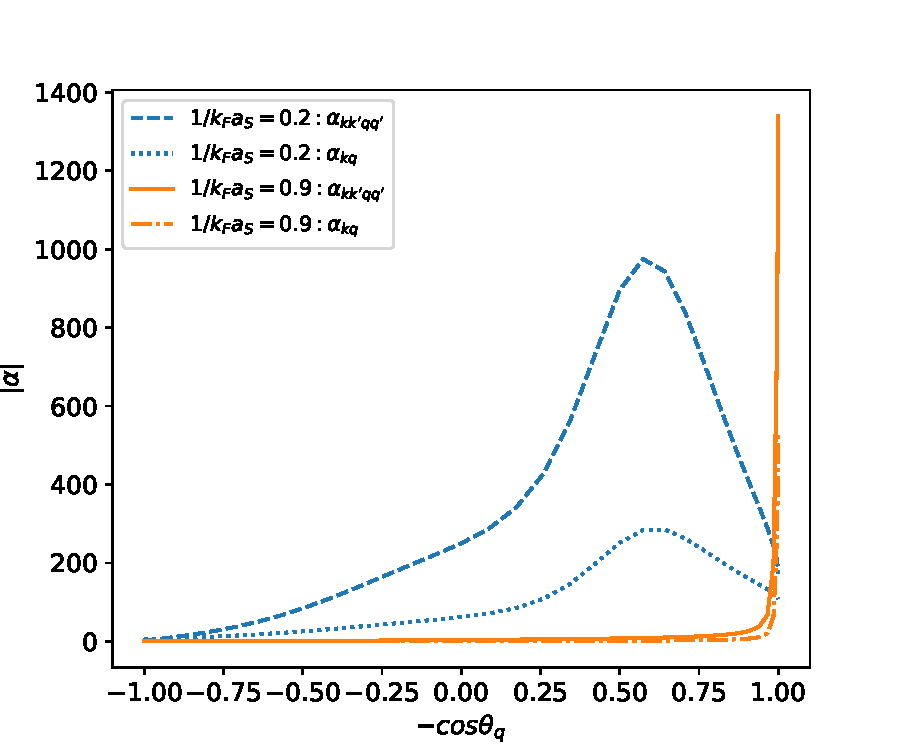
\includegraphics[width=0.7\textwidth]{fig3.pdf}
    \bicaption{铁磁($J>0$)与反铁磁($J<0$)耦合下整个体系平移对应的自旋单重态与自旋三重态能量后的能谱。其中a(1)代表能谱减掉$\frac{-9J^2}{8}$后的行为,b(1)代表了a(1)中灰色区域的放大。a(2)代表能谱减掉$\frac{-J^2}{8}$后的行为,可以看到基态依然随着$|J|$增大而能量越来越低,不再饱和到某一有限值。b(2)代表了a(2)中灰色区域的放大,从第一激发态开始,能量最终饱和在有限值。其中$E$与$J$的量纲为$\omega$与$\sqrt{\omega/M}$。}{a(1) Energies of deep bound states  for large and positive $J$, shifted by the spin-singlet binding energy $-9J^2/8$. All shifted energies saturate to a finite value, signifying the Kondo screening effect (see text).a(2) Energies of deep bound states  for large and negative $J$, shifted by the spin-triplet binding energy $-J^2/8$. The lowest bound state does not saturate as in b(1), showing the absence of screening effect for FM coupling. b(1,2) show the magnified plot for the shaded region in b(1,2), illustrating the asymptotic behavior towards odd harmonic levels. The units of $E$ and $J$ are respectively $\omega$ and $\sqrt{\omega/M}$.  }
    \label{fig:fig3}
\end{figure}

而在反铁磁情况下,基态branch的行为不同于铁磁情况。如图~\ref{fig:fig3}~a(2)所示,我们看到随着$J\to-\infty$,基态branch在减掉自旋三重束缚态二聚体能量$\frac{-J^2}{8}$之后依然越来越低,没有饱和在有限值。这表明此能量不仅由一个自旋三重束缚态贡献,剩下的那个费米子继续被二聚体所束缚,继续形成三体束缚态,导致能量进一步降低。除此之外,基态上面的激发态在减掉二聚体能量后最终趋向于有限的数值,如图~\ref{fig:fig3}~b(2)所示。

通过比较铁磁耦合与反铁磁耦合两种情况下基态的性质,我们发现对于一个杂质与两个费米子的1+2体系,铁磁耦合下,系统最多只能形成两体束缚态,局域的磁性杂质被一个费米子屏蔽之后无法再束缚更多的费米子。而对于反铁磁耦合,系统可以形成三体束缚态,局域杂质束缚了一个费米子之后还能继续束缚第二个费米子,导致能量比两体束缚态能量更低。这种特殊的少体关联效应是自旋交换相互作用所独有的。

为了进一步确认这种反铁磁耦合下系统的三体束缚态行为,我们考虑撤掉谐振子外势,考虑在一个一维自由体系,原点处固定一个自旋1/2的局域杂质,另有两个自旋1/2的全通费米子,长度为$L$,采用周期性边界条件,系统的哈密顿量为:
\begin{equation}
        \hat{H} = \sum_{j=1}^{2}  -\frac{1}{2M} \frac{\partial^2}{\partial x_{j}^2} + 2J\cdot\sum_{j=1}^2\delta(x_j){\hat{\Vector{S}}}_j\cdot {\hat{\Vector{S}}}.
\end{equation}
写在动量空间下的二次量子化哈密顿量为:
\begin{equation}\label{eq:free1+2}
\begin{split}
        \hat{H} &= \sum_{\Vector{k},\sigma}\epsilon_{\Vector{k},\sigma} \hat{C}^\dagger_{\Vector{k},\sigma} \hat{C}_{\Vector{k},\sigma}  + \sum_{\Vector{k}',\Vector{k}} \frac{J}{L} ( \hat{C}_{\Vector{k}'\uparrow}^\dagger  \hat{C}_{\Vector{k}\downarrow} \hat{S}_- + h.c. \\
        & \quad \quad +   (\hat{C}_{\Vector{k}'\uparrow}^\dagger  \hat{C}_{\Vector{k}\uparrow}-\hat{C}_{\Vector{k}'\downarrow}^\dagger  \hat{C}_{\Vector{k}\downarrow}) \hat{S}_{z} ).
\end{split}
\end{equation}
其中$\epsilon_{\Vector{k}} = \frac{\Vector{k}^2}{2M}$。在周期边界条件下,动量$\Vector{k} = \frac{2\pi\cdot n}{L}, n=0, \pm1, \pm2,...$。
在一维的情况下,对于纯接触势不需要做重整化,因此我们可以直接计算。由于方程(\ref{eq:free1+2})在形式上很类似于方程(\ref{eq:H2}),唯一的不同在于写在了不同的基矢表象下,对此我们依然采用矩阵对角化(\ref{final_eq})的办法,唯一的修改在于将其中的$\phi_m(0)$换为$\frac{1}{\sqrt{L}}$,$E_m$换为$\epsilon_{\Vector{k}}$,相应地,矩阵元变为:
\begin{equation}
\begin{split}
e_{kk'} &= \frac{1}{L}\frac{1}{E-E_k-E_{k'}}\\
q_{kk'} &= \delta_{kk'}  \frac{1}{L}\sum_p \frac{1}{E-E_k-E_p}\\
\end{split}
\end{equation}

在进行具体的数值计算之前,我们还需进一步讨论体系的特征尺度。在带有谐振子外势的体系中,系统有两个特征长度,分别是相互作用决定的$\frac{1}{MJ}$以及谐振子特征长度$\frac{1}{\sqrt{M\omega}}$。去掉谐振子之后的自由体系,仅有相互作用决定的特征长度$\frac{1}{MJ}$。因此我们用这个特征长度来做无量纲化,我们把具备这种特性的体系称为普适性体系。我们关心的物理是体系基态的束缚行为,对应的短程高能的物理,因此体系长度的选择于我们要考察的物理是不相关的,我们取足够大的动量截断$k_{\Lambda}/(MJ)=50$。{\color{red} 待补充 }

除了上面讨论的attractive branch的行为以外,我们还发现在能谱中有这样一类特殊的激发态。首先我们在能谱中将$S_{tot}=3/2$的态标记为红色。而且我们注意到这些$S_{tot}=3/2$的特殊态只在$J<0$的情况下成为lower attractive branch,在$J>0$的情况下趋向于有限值。如此特殊的行为也是很容易理解的,因为在$J>0$的区域,形成lower attractive branch的前提是其中一个费米子与杂质形成自旋单重二聚体束缚态,对应二聚体总的自旋为零,因此无法继续与剩下的费米子形成总自旋$S_{tot}=3/2$的自旋结构。由于自旋旋转对称性的保护,红色的$S_{tot}=3/2$与蓝色的$S_{tot}=1/2$的态之间永远正交,没有任何耦合,不会发生能级排斥现象。而且在$J>0$的情况下形成了upper repulsiev branch,我们称为铁磁repulsive branch。

如果我们仔细去考虑这支特殊的$S_tot=3/2$的铁磁branch的自旋部分,构型有三种:
\begin{equation}
    \begin{split} 
    |1\rangle &= |\uparrow\downarrow\Uparrow\rangle\\
    |2\rangle &= |\downarrow\uparrow\Uparrow\rangle\\
    |3\rangle &= |\uparrow\uparrow\Downarrow\rangle\\
    \end{split}
\end{equation} 
受到1+1中波函数自旋与空间分离的启发,其中铁磁要求任意一对自旋之间形成自旋三重态。我们构造$S_tot=3/2$的自旋波函数:
\begin{equation}
\Psi_{3,FM}(x_1,x_2)=\frac{1}{\sqrt{6}}\left|\begin{array}{cc}\psi_1(x_1) & \psi_1(x_2) \\\psi_2(x_1) & \psi_2(x_2)\end{array}\right| \left(|\uparrow\downarrow\Uparrow\rangle+|\downarrow\uparrow\Uparrow\rangle+|\uparrow\uparrow\Downarrow\rangle\right),
\end{equation}
其中自旋部分关于两个费米的自旋交换为对称,空间部分关于两个费米子交换为反对称。在这特殊的自旋构型下,相互作用中的自旋部分再一次地被对角化,自旋交换相互作用退化为纯的接触相互作用$U_t(x_i)=\gamma_t\delta(x_i)$,只影响波函数中的空间部分。其中$\psi_{1,2}$代表1+1体系中自旋三重态解的空间部分。我们巧妙的构造了这一特殊波函数,带入到薛定谔方程中:
\begin{equation}
\begin{split}
        \hat{H}\Psi_{3,FM}(x_1,x_2) = E\Psi_{3,FM}(x_1,x_2)\\
        E = E_1(J)+E_2(J)\\
\end{split}
\end{equation}
其中$E_1(J), E_2(J)$为1+1体系中自旋交换相互作用为$J$时候对应的自旋三重态本征能量。这时候三体体系是两体体系简单的相加。如果选取图~\ref{fig:fig2}~中三重态的基态与第一激发态,相加得到的三体能量即为铁磁态在整个相互作用区间的本征能量。$J\to-\infty$时,三体能量渐近行为是$E\to-\frac{J^2}{8}+1.5$;$J=0$时,$E=1.5+1.5=3$;$J\to\infty$时,$E\to1.5+3.5=5$。

值得一提的是,我们在自旋交换体系中发现的铁磁态与之前发现的自旋1/2费米子体系中的铁磁态\cite{cui2014ground}有很大不同,之前发现的铁磁态不会被s波相互作用所影响,其能量不随着相互作用变化。

除了上面讨论的铁磁态在$J>0$的时候是三体upper repulsive branch外,体系还有别的repulsive branch吗?要回答这个问题我们需要寻找能量随着相互作用$J\to\infty$而趋向于有限数值。我们仔细观察能谱,在能量$E=3\omega$附近有一支branch与能量不断降低的attractive branch发生能级排斥,$E=5\omega$附近有两条也发生能级排斥,发生能级排斥的位置最终逐渐饱和在有限值(随着$J\to\infty$能级排斥的能量区间越来越小,超过导致画图取点的分辨率),再加上已经发现的铁磁branch一共三条repulsive branch。受到铁磁态的启发,我们发现在$1/J=0$的极限情况下。铁磁态的波函数为
\begin{equation}
\Psi_{3,FM}(x_1,x_2)=\frac{1}{\sqrt{6}}\left|\begin{array}{cc}\psi_m(x_1) & \psi_n(x_2) \\\psi_m(x_1) & \psi_n(x_2)\end{array}\right| \left(|\uparrow\downarrow\Uparrow\rangle+|\downarrow\uparrow\Uparrow\rangle+|\uparrow\uparrow\Downarrow\rangle\right)
\end{equation}
其中$\psi_i(x)$为发生费米化之后谐振子的能级:
\begin{equation}
\psi_i(x) = \phi_{i}(x) \cdot sgn(x) 
\end{equation}
费米化之后的能级从低到高排布为:
\begin{equation}
E = 1.5\omega, 3.5\omega, 5.5\omega, ...
\end{equation}
如果选取最低的两个能级$E=1.5\omega, 3.5\omega$,恰好就是对应的铁磁态的能量。

但这仅仅是一支repulsive的能量,如何求解剩下的两支呢?由于1+2的三体体系存在内部的自旋结构,我们考虑费米子的全同交换反对称性,发现可以构造出三个三体波函数:
\begin{equation}
    \begin{split}
        &\left|\psi\right>^{(1)}_{deg} =  \frac{1}{\sqrt{2}} (\psi_1(x_1)\psi_3(x_2)- \psi_3(x_1)\psi_1(x_2)) \left|\uparrow \uparrow \Downarrow \right>\\
        &\left|\psi\right>^{(2)}_{deg} = \frac{1}{\sqrt{2}}\psi_1(x_1)\psi_3(x_2)\left|\uparrow \downarrow \Uparrow \right> - \frac{1}{\sqrt{2}}\psi_3(x_1)\psi_1(x_2)\left|\downarrow \uparrow \Uparrow \right>\\
        &\left|\psi\right>^{(3)}_{deg} = \frac{1}{\sqrt{2}}\psi_1(x_1)\psi_3(x_2)\left|\downarrow \uparrow \Uparrow \right> - \frac{1}{\sqrt{2}}\psi_3(x_1)\psi_1(x_2)\left|\uparrow \downarrow \Uparrow \right>\\
    \end{split}
\end{equation}
其中$\psi_i(x)$定义如前。这些波函数都满足$1/J=0$的情况下的边界条件:
\begin{equation}
    \psi(x_1\sigma_1,x_2\sigma_2) = 0 \quad \text{if} \quad x_i =0
\end{equation}
这表明,构造出的三个态是$1/J=0$时候体系简并态,简并的能量为$5\omega$。但是这仅仅是极限点处的三个本征态,当$1/J$成为非零的微扰项之后,此时upper branch的三重简并打开,这时候铁磁repulsive branch就是对应的打开简并后的零阶波函数。

基于这个图像,我们可以在1+2体系中再一次利用$1/J=0$附近的微扰论计算,去求解三支repulsuve branch的能量,这时候虽然与能谱上面降落下来的attractive branch仍有一定耦合,导致能级排斥现象的产生,但是这时候对应的attractive branch是非常深的束缚态,在空间上非常局域,这些态与repulsive branch的波函数交叠非常小,这大大提高了这些激发态的寿命,这一稳定性机理非常类似于{\color{red} upper branch实验观测待补充 },为实验室观察这些态创造良好的条件。具体地,我们假设这些简并态能量打开简并的方式如下:
\begin{equation}
    E_m(J) = E_0 - \frac{\kappa_m }{J} \quad \text{with}  \quad m =1,2,3  \label{E3m}
\end{equation}
对应的零阶波函数为之前构造简并波函数的线性叠加,叠加洗漱我们待定为$a_{mn}$:
    \begin{equation}
        \left|\psi^{(m)}_{\infty} \right> = \sum_n a_{mn} \left|\psi^{(n)}_{deg}\right>
    \end{equation}
当$1/J\neq=0$时候,我们假设这时候的本征repulsive branch波函数写为:
    \begin{equation}
        \begin{split}
            \left|\psi^{(m)}_J\right> &=  \psi^{(m)}_{J1}\left|\uparrow \uparrow \Downarrow \right> + \psi^{(m)}_{J2} \left|\uparrow \downarrow \Uparrow \right>  +\psi^{(m)}_{J3} \left|\downarrow \uparrow \Uparrow \right> \equiv\left(
            \begin{array}{c}
                \psi_{J1}^{(m)} \\
                \psi_{J2}^{(m)}\\
                \psi_{J3}^{(m)}
            \end{array}
            \right)\\
        \end{split} \label{eq2}
    \end{equation} 
自然地,当$1/J\to0$时候,我们有:
\begin{equation}\label{infcond}
    \lim_{1/J\to0} \left|\psi^{(m)}_J\right>  = \left|\psi^{(m)}_{\infty} \right>
\end{equation}
这将最终用来决定$a_{mn}$。
从方程(~\ref{E3m}~)的定义中,我们再一次利用Hellmann-Feynman定理得到$\kappa$满足:
    \begin{equation}
        \begin{split}
            \kappa_m \delta_{mn} &= \lim_{J\to \infty} \left<\psi^{(m)}_J\right| \frac{\partial\hat{H}}{\partial(\frac{-1}{J})} \left|\psi^{(n)}_{J}\right>\\
                &= \lim_{J\to \infty} \left<\psi^{(m)}_J\right| 2J^2(\delta(x_1)\hat{S_1}\cdot \hat{S_0}+\delta(x_2)\hat{S_2}\cdot \hat{S_0}) \left|\psi^{(n)}_{J}\right>\\
                &= \lim_{J\to \infty} \int  dx_2 \Psi^{(m)\dagger}_J(0,x_2) 2J^2 \hat{S_1}\cdot \hat{S_0} \Psi^{(n)}_J(0,x_2) \\
                &\quad + \int dx_1 \Psi^{(m)\dagger}_J(x_1,0) 2J^2 \hat{S_2}\cdot \hat{S_0} \Psi^{(n)}_J(x_1,0) \\
        \end{split} \label{kappam}
    \end{equation}
将$\left|\psi^{(m)}_J\right>$满足的薛定谔方程:
\begin{equation}
\hat{H} \left|\psi^{(m)}_J\right> = E_m(J)\left|\psi^{(m)}_J\right>
\end{equation}
左右两边分别对$x_1,x_2$求积分得到边界条件:
    \begin{equation}
        \begin{split}
            &\frac{1}{2M}\partial_{x_1} \Psi^{(m)}_J(x_1,x_2)|_{x_1=0^-}^{x_1=0^+}= 2J \hat{S_1}\cdot \hat{S_0}\Psi^{(m)}_J(0,x_2) \\
            &\frac{1}{2M}\partial_{x_2} \Psi^{(m)}_J(x_1,x_2)|_{x_2=0^-}^{x_2=0^+}= 2J \hat{S_2}\cdot \hat{S_0} \Psi^{(m)}_J(x_1,0)\\
        \end{split}
    \end{equation}
将上述边界条件满足的方程带入到方程(~\ref{kappam}~)中,然后取$J\to\infty$的极限,我们得到:
\begin{equation}\label{kappammid}
    \begin{split}
            \kappa_m \delta_{mn} &=  (\frac{1}{2M})^2 \int dx_2 \partial_{x_1} \Psi^{m\dagger}_{\infty}(x_1,x_2) |^{x_1=0^+}_{x_1 = 0^-} \frac{1}{2\hat{S_1}\cdot \hat{S_0}} \partial_{x_1} \Psi^{n}_{\infty}(x_1,x_2) |^{x_1=0^+}_{x_1 = 0^-}\\
            & \quad +  (\frac{1}{2M})^2 \int dx_1 \partial_{x_2} \Psi^{m\dagger}_{\infty}(x_1,x_2) |^{x_2=0^+}_{x_2 = 0^-} \frac{1}{2\hat{S_1}\cdot \hat{S_0}} \partial_{x_2} \Psi^{n}_{\infty}(x_1,x_2) |^{x_2=0^+}_{x_2 = 0^-}\\
    \end{split}
\end{equation} 
继而我们再带入之前假设的方程(~\ref{infcond}~)带入上式得到:
\begin{equation}
           \kappa_m \delta_{mn} = \frac{1}{M^2}(a_{m1},a_{m2},a_{m3}) \int dx
            \left(
            \begin{array}{c}
                \frac{4(B-A)^2}{3} \quad \frac{8B(B-A)}{3}  \quad \frac{8A(A-B)}{3}\\
                \frac{8B(B-A)}{3} \quad 4 A^2+\frac{4 B^2}{3}  \quad -\frac{16AB}{3} \\
                \frac{8A(A-B)}{3} \quad  -\frac{16AB}{3} \quad \frac{4 A^2}{3}+4 B^2
            \end{array}
            \right) 
            \left(
            \begin{array}{c}
                a_{n1}\\
                a_{n2}\\
                a_{n3}\\
            \end{array}
            \right)\\
\end{equation}
其中,我们记:
\begin{equation}
\begin{split}
A &= \frac{1}{\sqrt{2}}\phi_1'(0)\psi_3(x)\\
B &= \frac{1}{\sqrt{2}} \phi_3'(0)\psi_1(x)
\end{split}
\end{equation}
将具体函数带入并求积分:
\begin{equation}
\begin{split}
    \int dx A^2 &= \frac{(M\omega)^\frac{3}{2}}{\sqrt{\pi}}\\
    \int dx B^2 &= \frac{3 (M\omega)^\frac{3}{2} }{2\sqrt{\pi}} \\
    \int dx AB = 0
\end{split}
\end{equation}
最终将上式带入方程(~\ref{kappammid}~)得到:
\begin{equation}\label{kappammat}
    \kappa_m \delta_{mn} =  \omega \sqrt{\frac{\omega}{M}}\frac{1}{\sqrt{\pi}} \cdot(a_{m1},a_{m2},a_{m3})
            \left(
            \begin{array}{c}
                \frac{10}{3} \quad 4  \quad \frac{8}{3}\\
                4 \quad 6 \quad 0 \\
                \frac{8}{3} \quad 0 \quad \frac{22}{3}
            \end{array}
            \right) 
            \left(
            \begin{array}{c}
                a_{n1}\\
                a_{n2}\\
                a_{n3}\\
            \end{array}
            \right)   
\end{equation} 
由此关系,可以发现要求解的$\kappa_{m}$正好是方程右边矩阵的三个本征解,对应的本征矢量即为要求解的$a_{mn}$。

通过对角化方程(~\ref{kappammat}~)右边的矩阵,我们得到三个本征矢量(为归一化):
\begin{equation}
        \left(
            \begin{array}{c}
            1\\
            1\\
            1\\
            \end{array}
        \right),
        \left(
            \begin{array}{c}
            \frac{1}{2} \left(\sqrt{7}-3\right)\\
            \frac{1}{2} \left(1-\sqrt{7}\right)\\
            1\\
            \end{array}
        \right),
        \left(
            \begin{array}{c}
            \frac{1}{2} \left(-\sqrt{7}-3\right)\\
            \frac{1}{2} \left(\sqrt{7}+1\right)\\
            1\\
            \end{array}
        \right)\\
\end{equation}

其中第一个本征矢量恰好对应之前发现的铁磁态。与之相伴的本征值为(以$ \omega \sqrt{\frac{\omega}{M}}$为量纲):
\begin{equation}
\kappa_m= \frac{10}{\sqrt{\pi}},\frac{2}{3\sqrt{\pi}} \left(2 \sqrt{7}+5\right),\frac{2}{3\sqrt{\pi}} \left(5-2 \sqrt{7}\right) 
\end{equation}
我们将上述微扰论的结果与之前的严格对角化的数值结果进行比较,如图(~\ref{fig:fig4}~)所示,两种方法得到的能量行为一致。
\begin{figure}[!htbp]
    \centering
    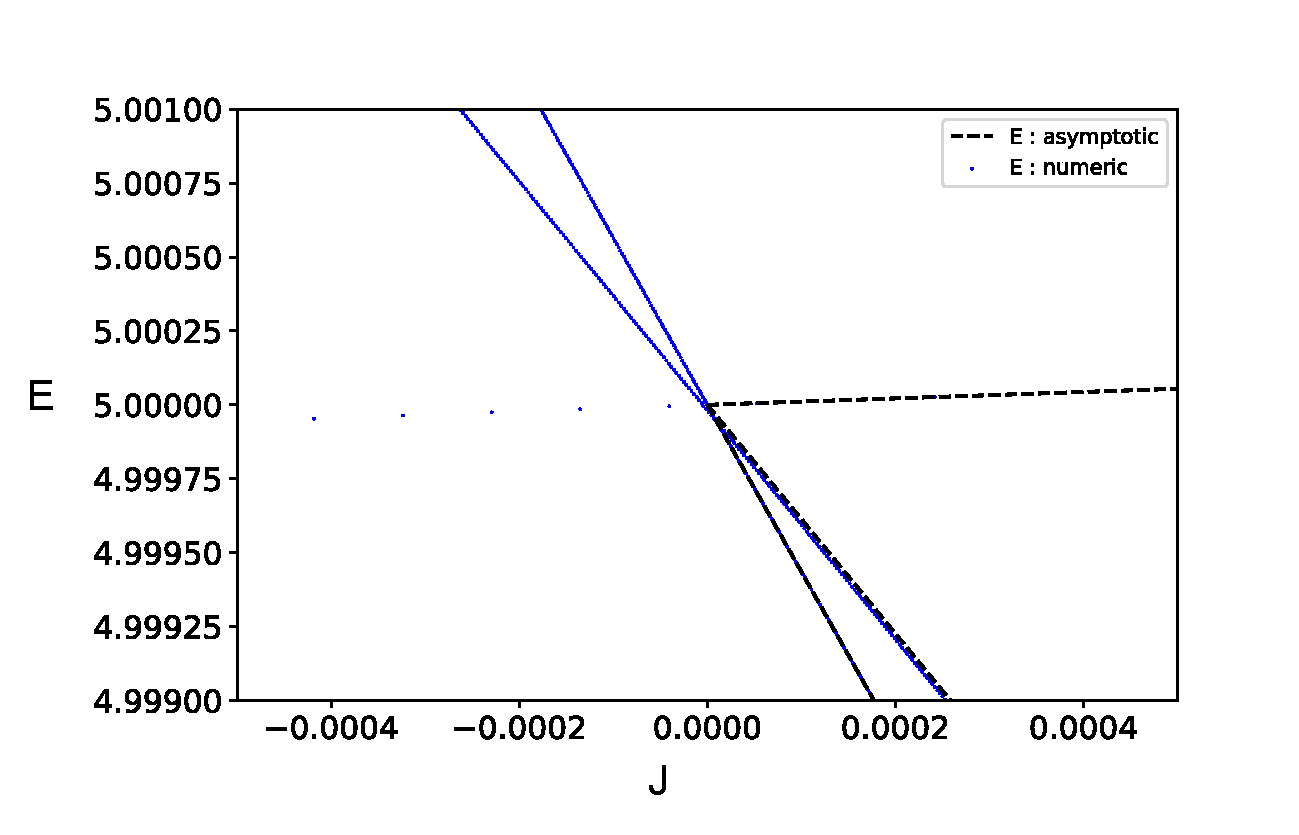
\includegraphics[width=0.7\textwidth]{fig4.pdf}
    \bicaption{能量$E=5\omega$附近三支repulsive branch的能量对比。其中蓝色散点图代表数值严格对角化的结果,黑色虚线代表$1/J=0$附近微扰论的结果。其中能量$E$与相互作用强度$J$的量纲为$\omega$和$\sqrt{\omega/M}$。}{Energy comparison of numerical exact diagonalization result and $1/J=0$ nearby perturbation result on repulsive branches aroud $E=5\omega$. Blue dotted line mark energy from perturbation and black dash line mark energy from numeric. The units of $E$ and $J$ are respectively $\omega$ and $\sqrt{\omega/M}$.  }
    \label{fig:fig4}
\end{figure}
以上讨论基于$E=5$附近的三支repulsive branch给出微扰计算,同样的方法可以应用到其余更高激发态上面去。综合上述讨论,我们完成了对能谱中强耦合条件下三体repsulsive 与 attractive branch的讨论,其中非平凡的关联效应进一步给出。我们在最后再讨论一下弱耦合下基态的行为。

在若耦合情况下$|J|\to0^{\pm}$,我们看到体系基态的能量行为,如图\ref{fig:fig2}~(a1,2)所示:
\begin{equation}
    E(J)\sim -cJ^2
\end{equation}
其随相互作用强固$J$变化的平方律的行为不同于纯接触势下线性律的行为,其原因在于极限情况下空间部分两个费米子占据谐振子的基态能级,自旋部分两费米子形成自旋单态,体系没有简并,一旦$J\neq0$,作为微扰项的自旋交换相互作用在基态上的期望值为零,这意味着平均场能量修正为零,最低阶的修正来自于二阶过程(从基态虚跃迁到高谐振子轨道)。

而对于弱耦合情况下的1+1体系的基态,单个费米子占据最低能级的谐振子轨道,微扰的自旋交换相互作用在其中的平均场贡献非零,导致能量的最低阶修正为随$J$的线性律。

中所周知,近藤模型在一定条件下可以用贝特假设的办法得到严格解\cite{Andrei-Furuya-Lowenstein}。在假设费米子的动能符合$\epsilon_{\Vector{k}}\propto|\Vector{k}|$的线性色散下,我们得到近藤模型基态的能量方程为:
\begin{equation}
    \begin{split}
        &\quad E_{gs}(J)-E_{gs}(J=0) \\
        &= D\cdot\left( \int\frac{1}{2c}\frac{\Theta(2\Lambda-2)-\pi}{\cosh\frac{\pi}{c}\Lambda}d\Lambda +i\ln\frac{1-\frac{iJ}{2}}{1+\frac{iJ}{2}} \right)
        \end{split}
\end{equation}
其中有:
\begin{equation}
    \begin{split}
    \Theta(x) &= -2\arctan(\frac{x}{c})\\
    c &= \frac{2J}{1-\frac{3J^2}{4}}\\
    \end{split}
\end{equation}
$D$是自由费米子的密度。相互作用$J$由$k_F/M$无量纲化。
这表明近藤模型基态的能量在$J\sim0$修正律为:
\begin{equation}
    E_{gs}(J)-E_{gs}(J=0) \propto J^3
\end{equation}
这与我们的少体1+1与1+2体系中的线性行为与平方行为都有很大的不同,对此的一个可能的解释在于我们的体系处在一个谐振子外势当中,谐振子的存在导致能级由自由空间的连续能级变为分立的谐振子能级。另外由于我们的体系是少体体系,少体中的弱耦合对应条件是$|J|\ll \sqrt{\omega/M}$(其中$\omega$为谐振子特征频率),近藤模型是多体体系,多体体系中弱耦合条件对应$|J|\ll \sqrt{E_F/M}$(其中$E_F$为多体体系的费米能量)。换句话讲少体体系的弱相互作用意味着自旋交换能量远小于单粒子激发的能隙,近藤模型中弱相互作用则要求自旋交换能量远小于费米能级,因此两种情况下的能量行为有较大不同。在{\color{red}附录}。
\section{小结与展望}\label{sec:spex-summary}

